\section{Conda ecosystem}
\subsection{a case of bioconda}

\begin{frame}{Conda system}
\begin{itemize}
\item \hyperlink{https://www.anaconda.com/}{Anaconda}
	\begin{itemize}
	\item Open source distribution
    \item Cross platform
    \item Available on cluster without admin whrite
    \item Thousands of available tool in informatic and bioinformatic
	\end{itemize}
\item \hyperlink{https://docs.conda.io/en/latest/miniconda.html}{Miniconda}
	\begin{itemize}
	\item A lightheight Anaconda version with minimal requirment
	\item Same advantages ad Anaconda
	\end{itemize}
\item \hyperlink{https://docs.conda.io/projects/conda/en/latest/index.html}{Conda}
	\begin{itemize}
	\item Package manager AND environment manager
	\item installed with Ana pr Miniconda
	\itme Python based but can also install tools from R, C++ or Julia...
	\end{itemize}
\end{itemize}
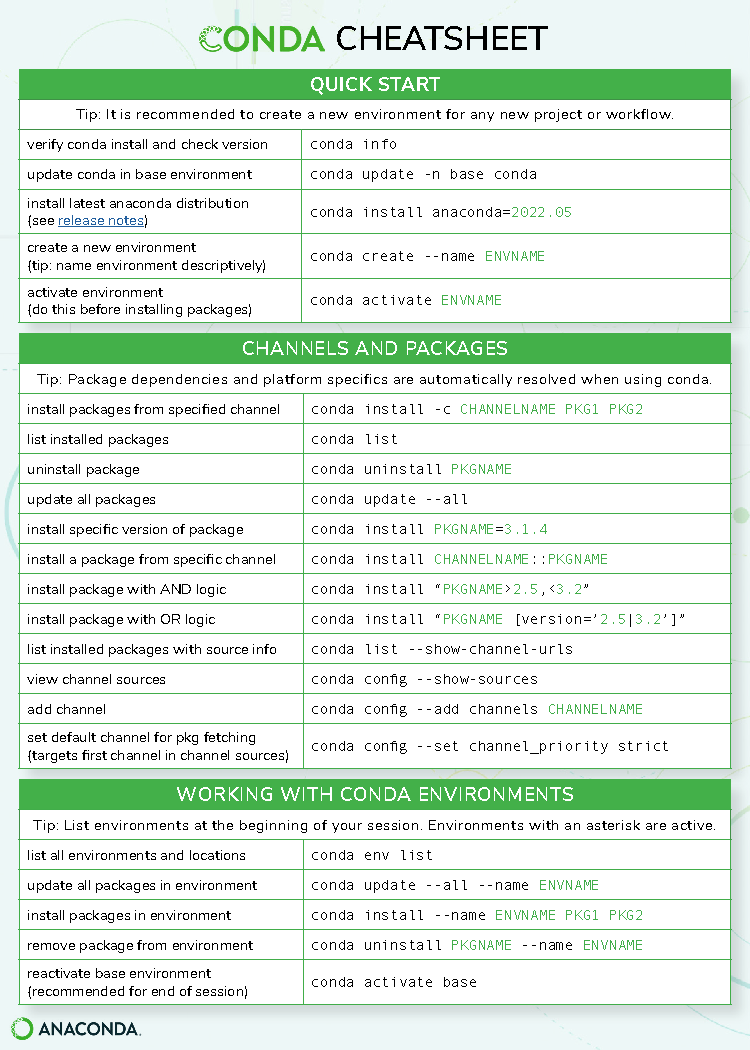
\includegraphics[width=0.1\textwidth]{images/conda_sheet_4.12.pdf} 

\includegraphics[width=0.1\textwidth]{images/conda_logo.pdf} 
\end{frame}

\begin{frame}{The channels and the tools}
The tools are packaged and available on several "channels"
\begin{itemize}
\item conda-forge
\item anaconda
\item R
\item Bioconda \footnote{Bioconda: sustainable and comprehensive software distribution for the life sciences \textit{Grüning et al.}, Nature methods, 2018. DOI 10.1038/s41592-018-0046-7}
	\begin{itemize}
	\item Most of the bioinformatic tools
	\end{itemize}
\end{itemize}
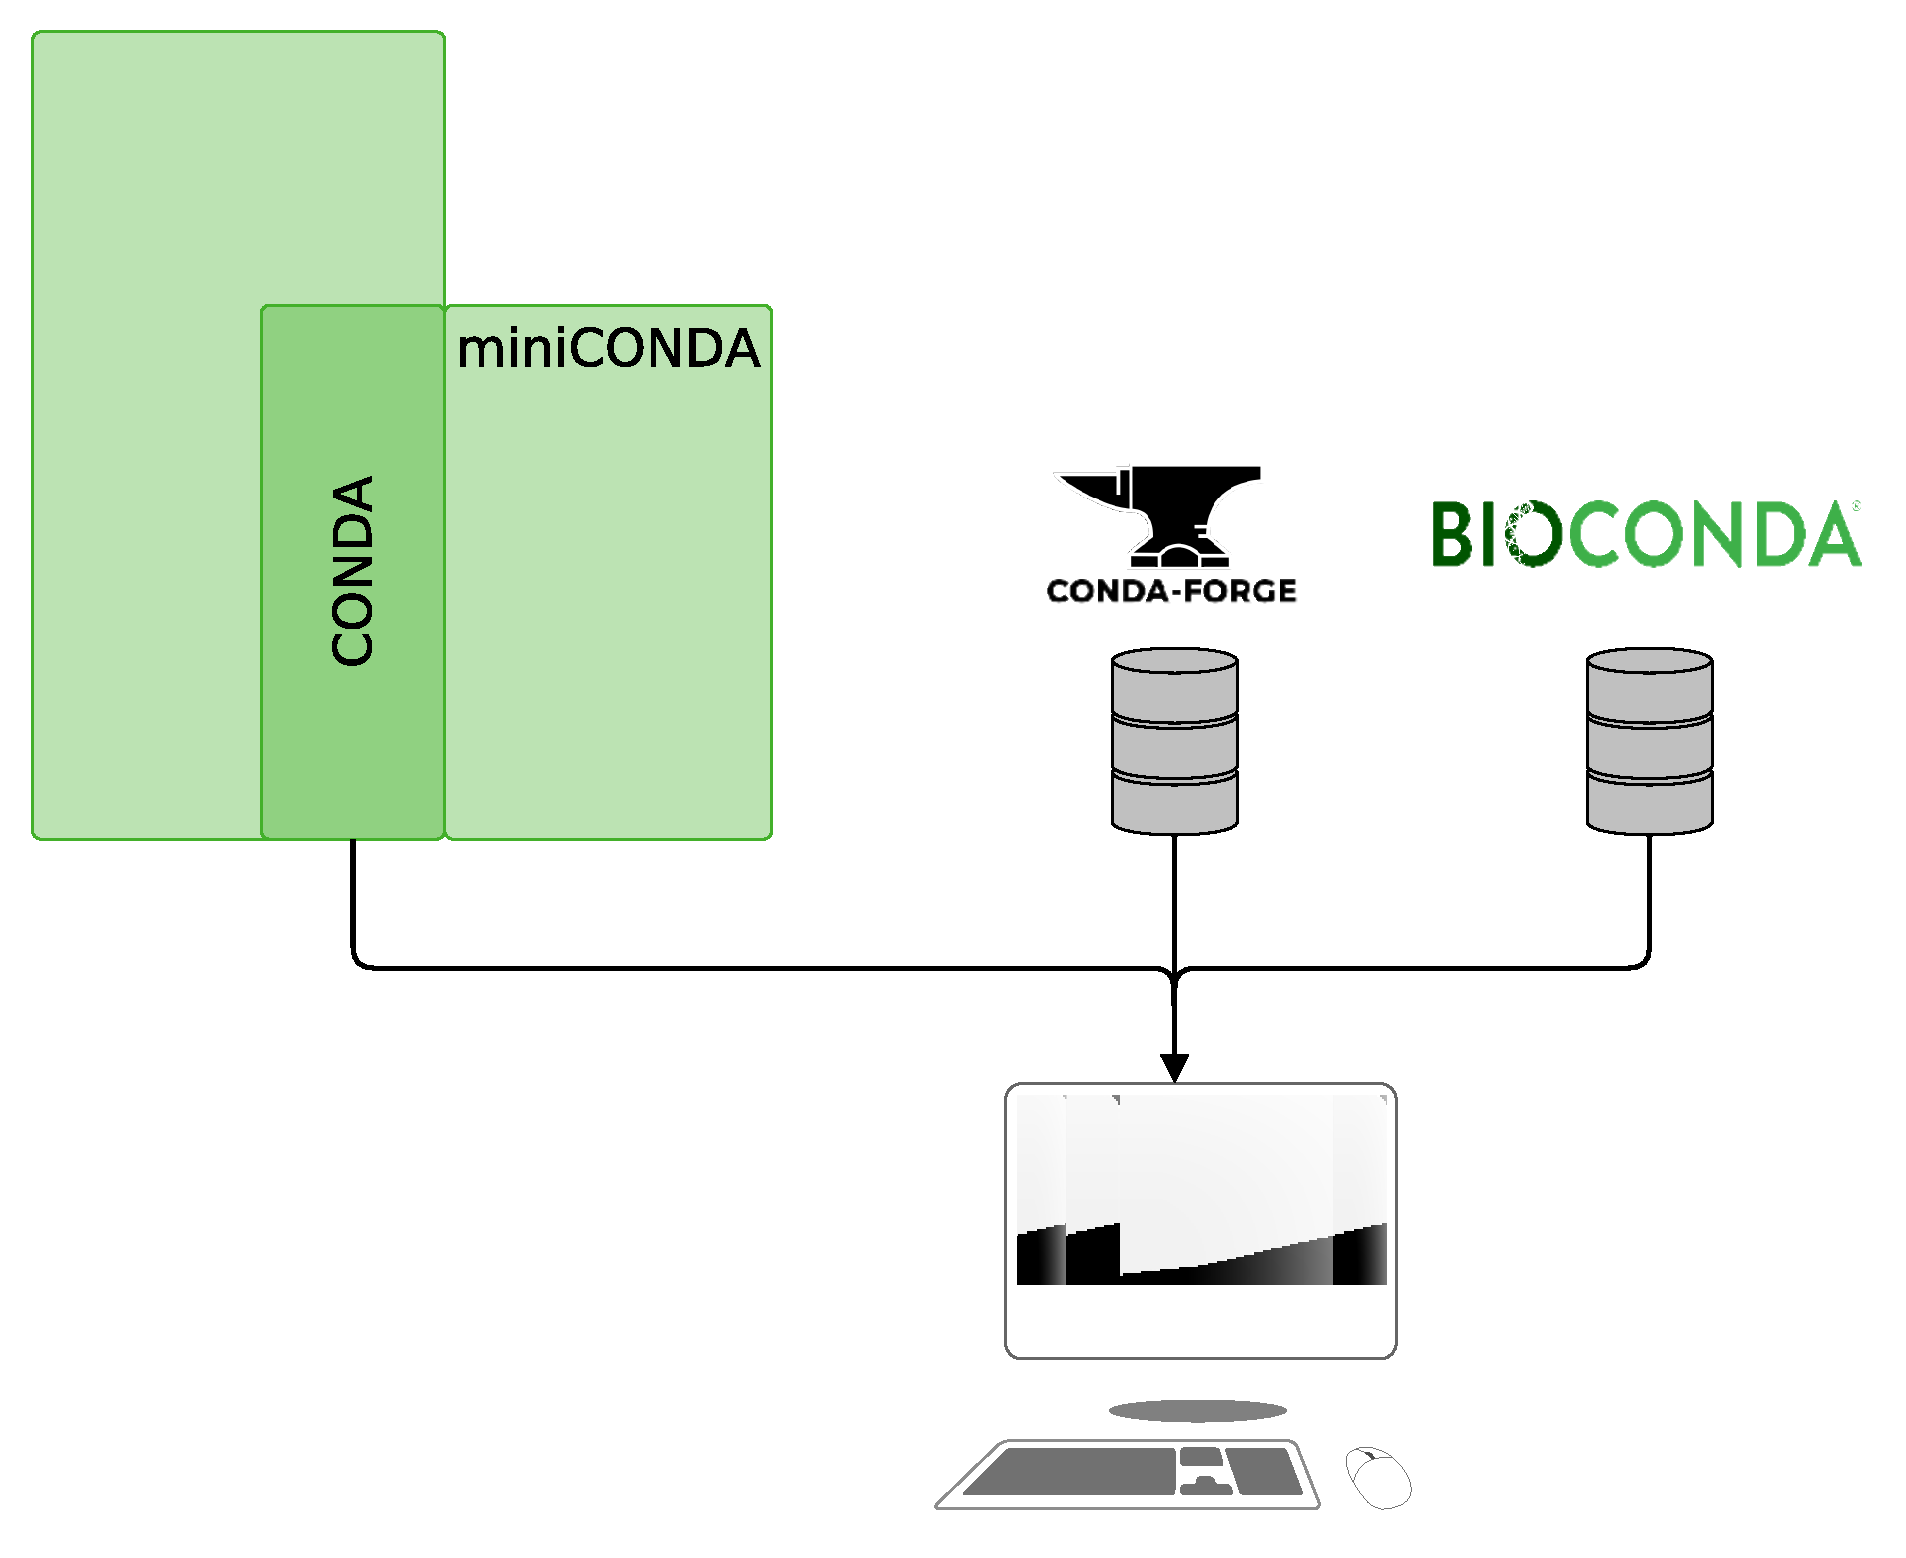
\includegraphics[width=0.1\textwidth]{images/conda_env_detail.pdf} 

\end{frame}